\section{Introduction}

Standard numerical methods tend to perform poorly across the board for the class of PDEs known as singular perturbation problems; these problems are often characterized by a parameter that may be either very small or very large.  An additional complication of singular perturbation problems is that very often, in the limiting case of the parameter blowing up or decreasing to zero, the PDE itself will change types (e.g.\ from elliptic to hyperbolic).  A canonical example of a singularly perturbed problem is the convection-diffusion equation in domain $\Omega \subset \mathbb{R}^3$,
\[
\div \left(\beta u\right) - \epsilon \Delta u = f.
\]
The equation models the steady-state distribution of the scalar quantity $u$, representing the concentration of a quantity in a given medium, taking into account both convective and diffusive effects. Vector $\beta \in \mathbb{R}^3$ specifies the direction and magnitude of convection, while the singular perturbation parameter $\epsilon$ represents the diffusivity of the medium. In the limit of an inviscid medium as $\epsilon\rightarrow 0$, the equation changes types, from elliptic to hyperbolic, and from second order to first order.

%We will illustrate the issues associated with numerical methods for this equation using one dimensional examples.  In 1D, the convection-diffusion equation is
%\begin{align*}
%\beta u'-\epsilon u'' &= f.
%\end{align*}
%For Dirichlet boundary conditions $u(0)=u_0$ and $u(1)= u_1$, the solution 
%can develop sharp boundary layers of width $\epsilon$ near the outflow boundary.
%\begin{figure}[!h]
%\centering
%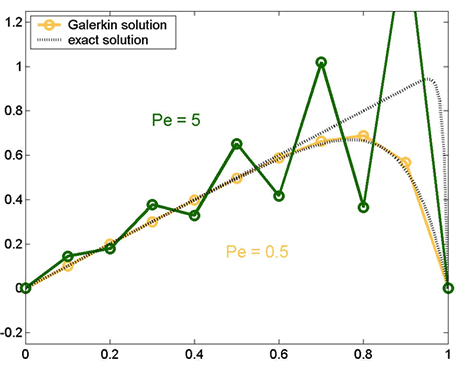
\includegraphics[width=2.5in]{figs/GalerkinOscTight.png}
%\caption{Oscillations in the 1D finite element solution of the convection-diffusion equation for small diffusion \cite{GalerkinOsc}. Standard finite volume and finite difference methods exhibit similar behavior.}
%\label{fig:GalerkinOsc}
%\end{figure}
The standard finite element method applied to the convection-dominated diffusion problem can perform very poorly for the case of small $\epsilon$.\footnote{This is especially true in the presence of boundary layers in the solution \cite{roos2008robust}.}  This poor performance can be observed numerically -- as the singular perturbation parameter $\epsilon$ decreases, the finite element solution can diverge significantly from the best finite element approximation of the solution.  
%The poor performance of the finite element method for this problem is reflected in the bound on the error in the finite element solution --- under the standard Bubnov-Galerkin method with $u\in H^1(0,1)$, we have the bound given in \cite{roos2008robust}:
%\[
%\|u-u_h\|_\epsilon \leq C \inf_{w_h}\|u-w_h\|_{H^1(0,1)},
%\]
%for $\|u\|_\epsilon^2 \coloneqq \|u\|_{L^2}^2 + \epsilon \|u'\|_{L^2}^2$, with $C$ independent of $\epsilon$. An alternative formulation of the above bound is 
%\[
%\|u-u_h\|_{H^1(0,1)} \leq C(\epsilon) \inf_{w_h}\|u-w_h\|_{H^1(0,1)},
%\]
%where $C(\epsilon)$ grows as $\epsilon\rightarrow 0$. The dependence of the constant $C$ on $\epsilon$ is what we refer to as a \textit{loss of robustness} --- as the singular perturbation parameter $\epsilon$ decreases, our finite element error is bounded more and more loosely by the best approximation error.  As a consequence, the finite element solution can diverge significantly from the best finite element approximation of the solution for very small values of $\epsilon$.  
For example, it is well known that, on a fixed coarse mesh and for small values of $\epsilon$ (or a large Peclet number, the ratio $h/\epsilon$), the Galerkin approximation of the solution to the convection-diffusion equation with a boundary layer develops spurious oscillations everywhere in the domain, even where the best approximation error is small.  These oscillations grow in magnitude as $\epsilon \rightarrow 0$, eventually polluting the entire solution.\footnote{For nonlinear shock problems, the solution often exhibits sharp gradients or discontinuities, around which the solution would develop spurious Gibbs-type oscillations. These are a result of underresolution of the solution, and are separate from the oscillations resulting from a lack of robustness.}  

Traditionally, instability/loss of robustness in finite element methods has been dealt with using residual-based stabilization techniques.  Given some variational form, the problem is modified by adding to the bilinear form the strong form of the residual, weighted by a test function and scaled by a stabilization constant $\tau$.  The most well-known example of this technique is the streamline-upwind Petrov-Galerkin (SUPG) method, which is a stabilized FE method for solving the convection-diffusion equation using piecewise linear continuous finite elements \cite{SUPG}.  SUPG stabilization not only removes the spurious oscillations from the finite element solution of the convection-diffusion equation, but delivers the best finite element approximation in the $H^1$ norm in 1D.  

From the perspective of the compressible Navier-Stokes equations, this loss of robustness is doubly problematic.  Not only will any nonlinear solution suffer from similar unstable oscillations, but nonlinear solvers themselves may fail to yield a solution due to such instabilities.  A nonlinear solution is almost always computed by solving a series of linear problems whose solutions will converge to the nonlinear solution under appropriate assumptions, and the presence of such oscillations in each linear problem can cause the solution convergence to slow significantly or even diverge.  Artificial viscosity and shock capturing methods have been used to suppress such oscillations and regularize the problem.  While these methods will usually yield smooth and qualitatively resolved solutions, these methods are often overly diffusive, yielding results which are poor approximations of the true solution \cite{Gresho1981223}, though modern artificial viscosity and shock capturing schemes have improved greatly in recent years \cite{Barter,Guermond20114248}.  We have taken an alternative approach in this work, avoiding artificial diffusion and shock capturing for the moment.  

Our aim is to develop a stable, higher order scheme for the steady compressible laminar Navier-Stokes equations in transonic/supersonic regimes that is automatically adaptive beginning with very coarse meshes.  This requires that both the method and the refinement scheme to perform adequately on coarse meshes with high Peclet numbers -- in other words, that the adaptive method is robust in the diffusion parameter.  We construct such a method in this paper as follows: we begin by deriving the DPG method for linear problems, then constructing a DPG method for the scalar convection-diffusion equation that is robust for very small viscosities.  Unlike common adaptive methods in computational fluid dynamics, which often refine based on physical features (such as high gradients in the solution), adaptivity under this method is driven by the minimization of a residual, which measures error accurately even for highly underresolved meshes.  The DPG method for scalar convection-diffusion is then extrapolated to systems of nonlinear equations, and applied to the compressible Navier-Stokes equations.  Numerical experiments are given, demonstrating the robustness of the method and the effectiveness of automatic adaptivity for two model problems in viscous compressible flow. 
